\apendice{Documentación de usuario}

\section{Introducción}

\section{Requisitos de usuarios}
En este apartado se detallarán las especificaciones mínimas tanto software como hardware que se requerirán para un correcto funcionamiento de la aplicación.
\subsection{Requisitos hardware}
Podemos diferenciar dos posibles formas de ejecutar la aplicación: a través de un emulador \textit{Android} instalado en un PC y a través de un dispositivo móvil con sistema operativo \textit{Android}.
\begin{itemize}
\item \textbf{Emulador en un PC:} será necesario que el PC tenga instalados tanto el compilador \textit{Java} como un emulador  con el SDK de \textit{Android}.
Se recomienda que el emulador utilizado sea \textit{Android Emulator API 23}.
Este emulador tiene sus propias restricciones hardware, que son:
\begin{itemize}
\item Procesador de 64 bits. \textit{Android Emulator} NO se encuentra disponible para procesadores de 32 bits desde Junio/2019
\item SDK Tools 26.1.1 (o posterior)
\item HAXM 6.2.1 o posterior (aunque se recomienda HAXM 7.2.0 o posterior)
\item Procesador \textit{Intel} i3, i5 o i7. Se ha observado que aunque es posible utilizar procesadores \textit{AMD}, se recomienda que estos sean actuales ya que en un principio el emulador se probó con un procesador \textit{AMD ryzen2700x} y no funcionó.
\end{itemize}
\item \textbf{Dispositivo móvil:} se podrá utilizar cualquier dispositivo (móvil o tablet) que cuente con \textit{Android 6.0} o superior. La aplicación se ha instalado y ejecutado en un dispositivo \textit{Google Pixel 2} y un \textit{BQ Aquaris E5} y en ambos ha dado buenos resultados.
\end{itemize}
\subsection{Requisitos software}
Los requisitos software son los siguientes:
\begin{itemize}
\item Compilador \textit{Java}. Necesario para programar aplicaciones \textit{Android} y ejecutar la máquina virtual de \textit{Java} (JVM)
\item \textit{Android Studio}, desarrollado por \textit{Google}, que nos permite desarrollar y ejecutar aplicaciones para la plataforma \textit{Android}
\item \textit{Oracle Glassfish Server 3}, que contendrá el servidor encargado de las respuestas a las peticiones del cliente.
\item \textit{Oracle VM VirtualBox}, utilizado en caso de no querer instalar los programas mencionados anteriormente. Bastaría con cargar la máquina virtual con el cliente/servidor. Cabe destacar que en caso de que el ordenador no tenga demasiada potencia es posible que \textit{VirtualBox} no sea capaz de funcionar correctamente.
\end{itemize}
\section{Instalación}
En esta sección se encuentra detallada la guía de instalación de la aplicación.

Cabe destacar que es necesario instalar tanto el cliente en un dispositivo \textit{Android} ( o emulador) como el servidor en \textit{Glassfish}.
\subsection{Instalación de la aplicación en el servidor}
Debido a que la versión de \textit{Glassfish} utilizada es la misma que en anteriores versiones del proyecto, se seguirán los mismos pasos para la instalación del servidor. Dichos pasos son los siguientes:

Para instalar la aplicación en el servidor, hay que abrir la consola de administración de \textit{GlassFish} tecleando en un navegador web la dirección del servidor con el puerto 4848 (http://localhost:4848 en este caso) e ir a la opción \textit{Applications}.

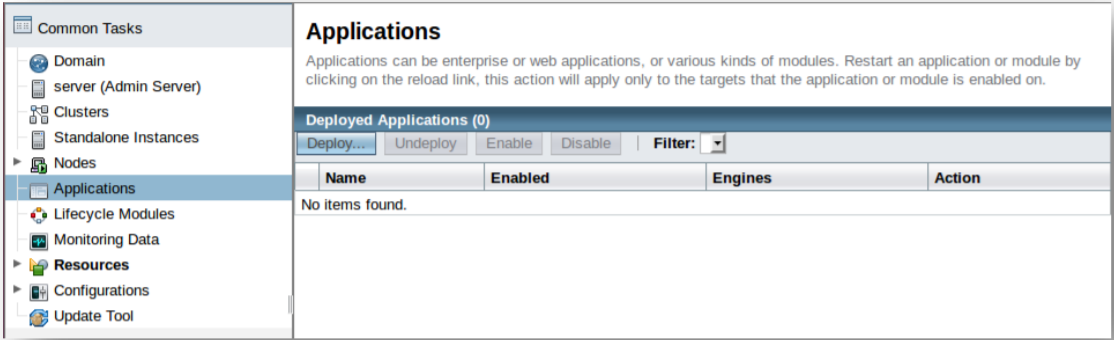
\includegraphics[width=\textwidth]{C5_InSer1}

A continuación hay que hacer \textit{click} sobre el botón \textit{Deploy} e indicar la ruta en la que se encuentra el archivo \textit{.war} , después una vez que se haga \textit{click} sobre el botón OK ya estará la aplicación publicada y funcionando.

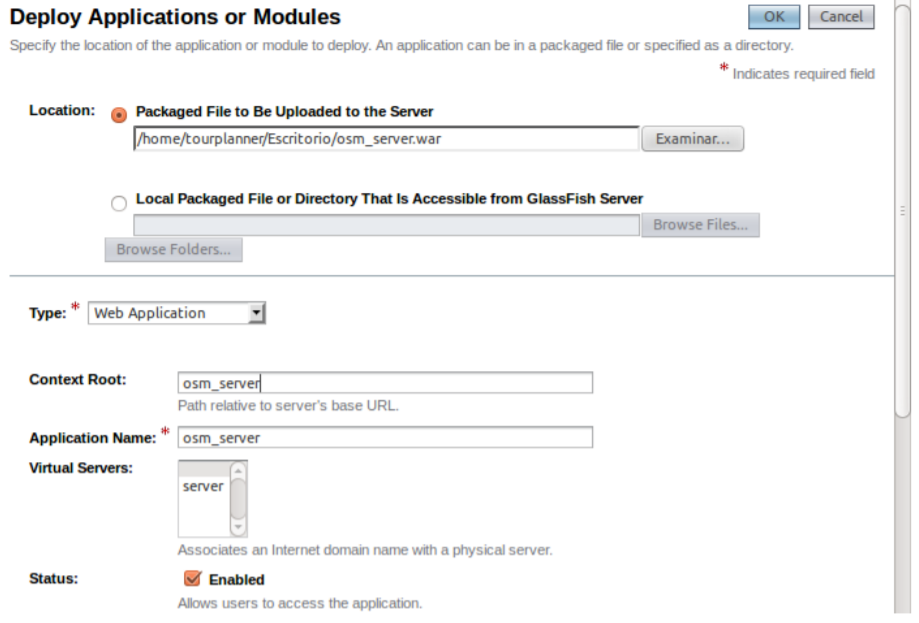
\includegraphics[width=\textwidth]{C5_InSer2}


\subsection{Instalación de la aplicación en el cliente}
Para realizar la instalación de nuestra aplicación \textit{Android} en un dispositivo físico o un emulador necesitaremos seguir los siguientes pasos:
\begin{itemize}
\item En caso de un dispositivo físico será necesario que éste se encuentre conectado al sistema en el que tengamos la aplicación.
\item Una vez tengamos lista la aplicación pulsaremos el botón de \textit{Play} en \textit{Android Studio}.

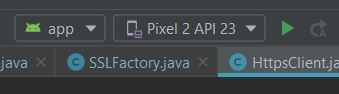
\includegraphics[width=\textwidth]{C5_installAndroid}

\item \textit{Android Studio} será el encargado de instalar el archivo \textit{.apk} dentro del dispositivo y lo ejecutará automáticamente.

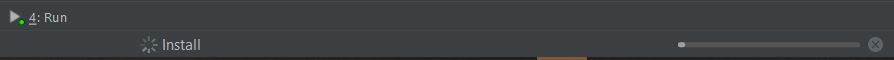
\includegraphics[width=\textwidth]{C5_PlayAn}

\textbf{AC: ACTUALIZAR SEGUN MANUAL DE SUSO}
Hay que tener en cuenta que para el correcto funcionamiento de la aplicación hay que seguir correctamente los pasos de compilación explicados en el apartado \textit{Compilación del cliente}, prestando especial atención al punto en el que se establece la dirección IP y puerto del servidor.

\end{itemize}
\subsection{Ejecución de la aplicación}
Para lograr que la aplicación se ejecute correctamente sin la necesidad de contar con un servidor y un cliente independientes, se han incluido en el USB del proyecto las máquinas virtuales correspondientes a el cliente y el servidor. De esta forma podremos ejecutar la aplicación con un solo ordenador.

Cabe destacar que para lograr que ambas máquinas virtuales se comuniquen entre sí correctamente, se ha utilizado el programa \textit{LogMeIn Hamachi} que nos permite crear redes virtuales entre ambas máquinas a través de Internet.
\subsubsection{Ejecución de la aplicación servidor}
Para ejecutar la aplicación servidor, se importa la máquina virtual \textit{Servidor-Ubuntu 18.04 LTS} en \textit{VirtualBox} (hay más software de creación de máquinas virtuales pero este es el que se ha utilizado).

\textbf{AC: FOTO}

\subsubsection{Ejecución de la aplicación cliente}
Para ejecutar la aplicación cliente, al igual que con la aplicación servidor, se importa la máquina virtual \textit{Cliente-Windows 10} en \textit{VirtualBox}.

Una vez se haya iniciado la máquina virtual, se hace doble \textit{click} sobre el entorno de desarrollo \textit{Android Studio}. A continuación, hacemos doble \textit{click} sobre el icono \textit{Play}.

\textbf{AC: FOTO}

\section{Manual del usuario}


